\documentclass[conference]{IEEEtran}

% =========================================================
% PARÁMETROS CONFIGURABLES POR SEMANA
% =========================================================
\newcommand{\NumeroSemana}{08}
\newcommand{\TemaSemana}{APLICACIONES DEL TEOREMA FUNDAMENTAL DEL CÁLCULO}

% --- PAQUETES BÁSICOS Y MATEMÁTICOS ---
\usepackage[utf8]{inputenc}
\usepackage[T1]{fontenc}
\usepackage{amsmath,amssymb,amsfonts}
\usepackage{mathtools}
\usepackage{graphicx}
\usepackage{hyperref}
\usepackage{float}
\usepackage{array}

% --- RUTA BÁSICA DE IMÁGENES ---
\graphicspath{{semana_05/graficas/}}

\begin{document}
	
	% =========================================================
	% PORTADA OFICIAL FORMATO IEEE - FIEE UNMSM
	% =========================================================
	\title{UNIVERSIDAD NACIONAL MAYOR DE SAN MARCOS\\
		\Large FACULTAD DE INGENIERÍA ELECTRÓNICA Y ELÉCTRICA (FIEE)\\
		\vspace{0.3cm}
		\large \textbf{Curso:} Cálculo II (Cálculo Integral) \quad|\quad \textbf{Docente:} Dr. Raúl Castro Vidal\\
		\vspace{0.4cm}
		\huge SOLUCIÓN DE EJERCICIOS PROPUESTOS --- SEMANA \NumeroSemana\\
		\LARGE INFORME TÉCNICO GRUPAL: \TemaSemana}
	
	% --- BLOQUE DE AUTORES ---
	\author{
		\IEEEauthorblockN{Coordinador: Adrián Córdova Suazo}
		\IEEEauthorblockA{\textit{Código: 26190164} \\
			\textit{Ing. Electrónica}}
		\and
		\IEEEauthorblockN{Integrante 2: Diego Checcori Cuya}
		\IEEEauthorblockA{\textit{Código: 26190008} \\
			\textit{Ing. Electrónica}}
		\and
		\IEEEauthorblockN{Integrante 3: Diego Anamaria Choque}
		\IEEEauthorblockA{\textit{Código: 26190001} \\
			\textit{Ing. Electrónica}}
		\vspace{0.4cm}
		\and
		\IEEEauthorblockN{Integrante 4: Deyvis Tenorio Yucra}
		\IEEEauthorblockA{\textit{Código: 26190199} \\
			\textit{Ing. Electrónica}}
		\and
		\IEEEauthorblockN{Integrante 5: Felix Chocce Oseda}
		\IEEEauthorblockA{\textit{Código: 23190231} \\
			\textit{Ing. Eléctrica}}
		\and
		\IEEEauthorblockN{Integrante 6: Isaac Guadalupe Baños}
		\IEEEauthorblockA{\textit{Código: 26190169} \\
			\textit{Ing. Electrónica}}
	}
	
	\maketitle
	
	\begin{abstract}
		En el presente informe técnico correspondiente a la asignatura de Cálculo II, a cargo del Dr. Raúl Castro Vidal, se presenta la solución analítica paso a paso de los ejercicios propuestos para la Semana \NumeroSemana. Cada problema incluye su representación y análisis gráfico desarrollado en Matplotlib evaluado en la constante de integración $C=0$, estructurado formalmente bajo los estándares IEEE a dos columnas.
	\end{abstract}
	
	\begin{IEEEkeywords}
		Cálculo II, \TemaSemana, Matplotlib, Formato IEEE, FIEE-UNMSM.
	\end{IEEEkeywords}
	
	\section{Desarrollo de los Ejercicios}
	
	% --- LISTA DIRECTA CON RUTAS EXPLÍCITAS ---
	\subsection*{Problema 01}

\textbf{Enunciado:} Probar que:
\begin{align*}
\lim_{x \to \infty} \dfrac{\ln(x)}{x} = 0 \quad \text{y} \quad \lim_{x \to 0^+} \ln(x) = -\infty
\end{align*}

\textbf{Solución:}
Para la primera parte, evaluamos el límite
\begin{align*}
\lim_{x \to \infty} \dfrac{\ln(x)}{x}
\end{align*}
el cual presenta la forma indeterminada $\frac{\infty}{\infty}$. Aplicando la regla de L'Hôpital, derivamos el numerador y el denominador respecto a $x$:
\begin{align*}
\lim_{x \to \infty} \dfrac{\frac{d}{dx}[\ln(x)]}{\frac{d}{dx}[x]} &= \lim_{x \to \infty} \dfrac{\frac{1}{x}}{1} \\
&= \lim_{x \to \infty} \dfrac{1}{x} = 0
\end{align*}
Con esto queda demostrado el primer límite.

Para la segunda parte, evaluamos el límite cuando $x$ tiende a $0^+$ del logaritmo natural:
\begin{align*}
\lim_{x \to 0^+} \ln(x)
\end{align*}
Aplicamos el cambio de variable sugerido haciendo $x = \dfrac{1}{t}$. 
Cuando $x \to 0^+$, la variable $t$ tiende a la infinidad positiva ($t \to \infty$). 
Sustituyendo en la expresión original, tenemos:
\begin{align*}
\lim_{x \to 0^+} \ln(x) &= \lim_{t \to \infty} \ln\left(\dfrac{1}{t}\right) \\
&= \lim_{t \to \infty} \left[ \ln(1) - \ln(t) \right]
\end{align*}
Sabemos que $\ln(1) = 0$, por lo que la expresión se reduce a:
\begin{align*}
\lim_{t \to \infty} \left[ 0 - \ln(t) \toBe} &= -\lim_{t \to \infty} \ln(t) \\
&= -\infty
\end{align*}
Esto completa la demostración de ambos límites solicitados.

\begin{figure}[H]
	\centering
	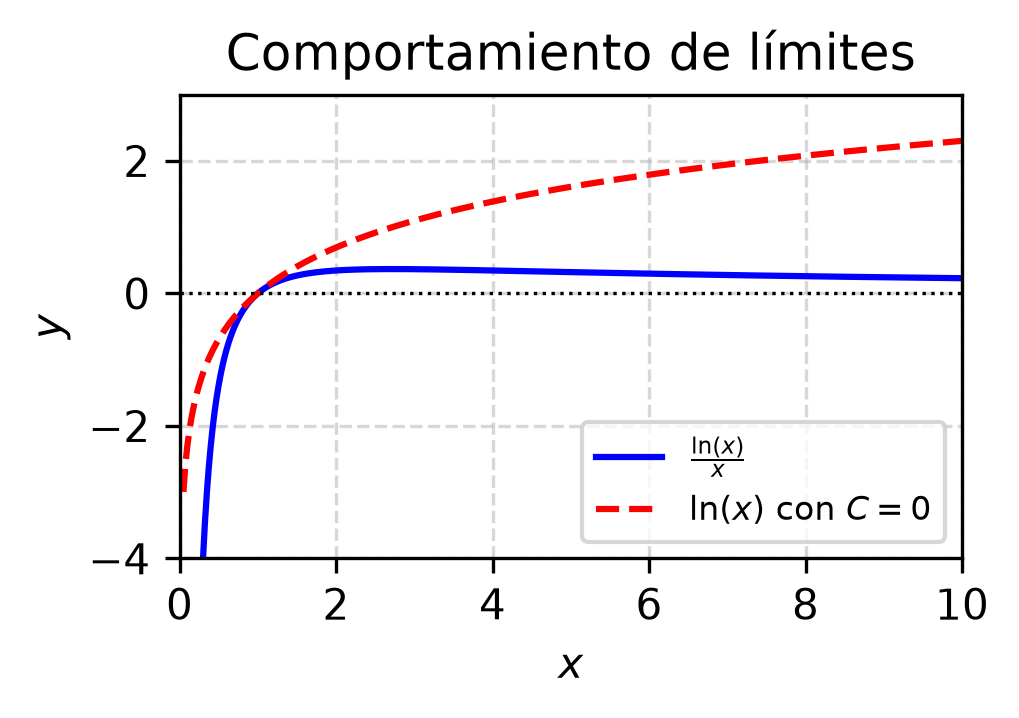
\includegraphics[width=\columnwidth]{semana_08/graficas/SEM08_P01_grafica.png}
	\caption{Representación gráfica de $f(x)$ y su antiderivada $F(x)$ evaluada para la constante de integración $C = 0$ (Problema 01).}
	\label{fig:problema01}
\end{figure}

	\subsection*{Problema 02}

\noindent\textbf{Enunciado:} 
Probar que si $x < 1$ (con $x > 0$), entonces se cumple que $\ln(x) < x$.

\noindent\textbf{Solución:}
Para demostrar la desigualdad propuesta, definimos una función auxiliar en todo el dominio $x > 0$ tal que:

\begin{align*}
    f(x) &= x - \ln(x)
\end{align*}

El objetivo es analizar el comportamiento de esta función y determinar su valor mínimo absoluto para $x > 0$. Para ello, calculamos la primera derivada de $f(x)$ respecto a $x$:

\begin{align*}
    f'(x) &= \dfrac{d}{dx} \left[ x - \ln(x) \right] \\
    f'(x) &= 1 - \dfrac{1}{x}
\end{align*}

Igualamos la derivada a cero para encontrar los puntos críticos en el dominio $x > 0$:

\begin{align*}
    1 - \dfrac{1}{x} &= 0 \\
    1 &= \dfrac{1}{x} \\
    x &= 1
\end{align*}

El único punto crítico ocurre en $x = 1$. Evaluamos la segunda derivada para determinar la naturaleza de este punto crítico:

\begin{align*}
    f''(x) &= \dfrac{d}{dx} \left[ 1 - \dfrac{1}{x} \right] \\
    f''(x) &= \dfrac{1}{x^2}
\end{align*}

Evaluando en el punto crítico $x = 1$:

\begin{align*}
    f''(1) &= \dfrac{1}{(1)^2} = 1 > 0
\end{align*}

Dado que la segunda derivada es positiva en $x = 1$, por el criterio de la segunda derivada, $f(x)$ tiene un mínimo absoluto en dicho punto. Calculamos el valor de la función en este mínimo:

\begin{align*}
    f(1) &= 1 - \ln(1) \\
    f(1) &= 1 - 0 = 1
\end{align*}

Como $f(1) = 1$ es el valor mínimo de la función para todo $x > 0$, se concluye que la función es estrictamente positiva en todo su dominio:

\begin{align*}
    f(x) &\ge 1 > 0 \quad \text{para todo } x > 0
\end{align*}

Sustituyendo la definición original de $f(x)$, obtenemos:

\begin{align*}
    x - \ln(x) &> 0 \\
    x &> \ln(x)
\end{align*}

Invirtiendo la desigualdad, queda demostrado que:

\begin{align*}
    \ln(x) &< x \quad \text{para todo } x < 1 \text{ (con } x > 0\text{)}
\end{align*}

\begin{figure}[H]
    \centering
    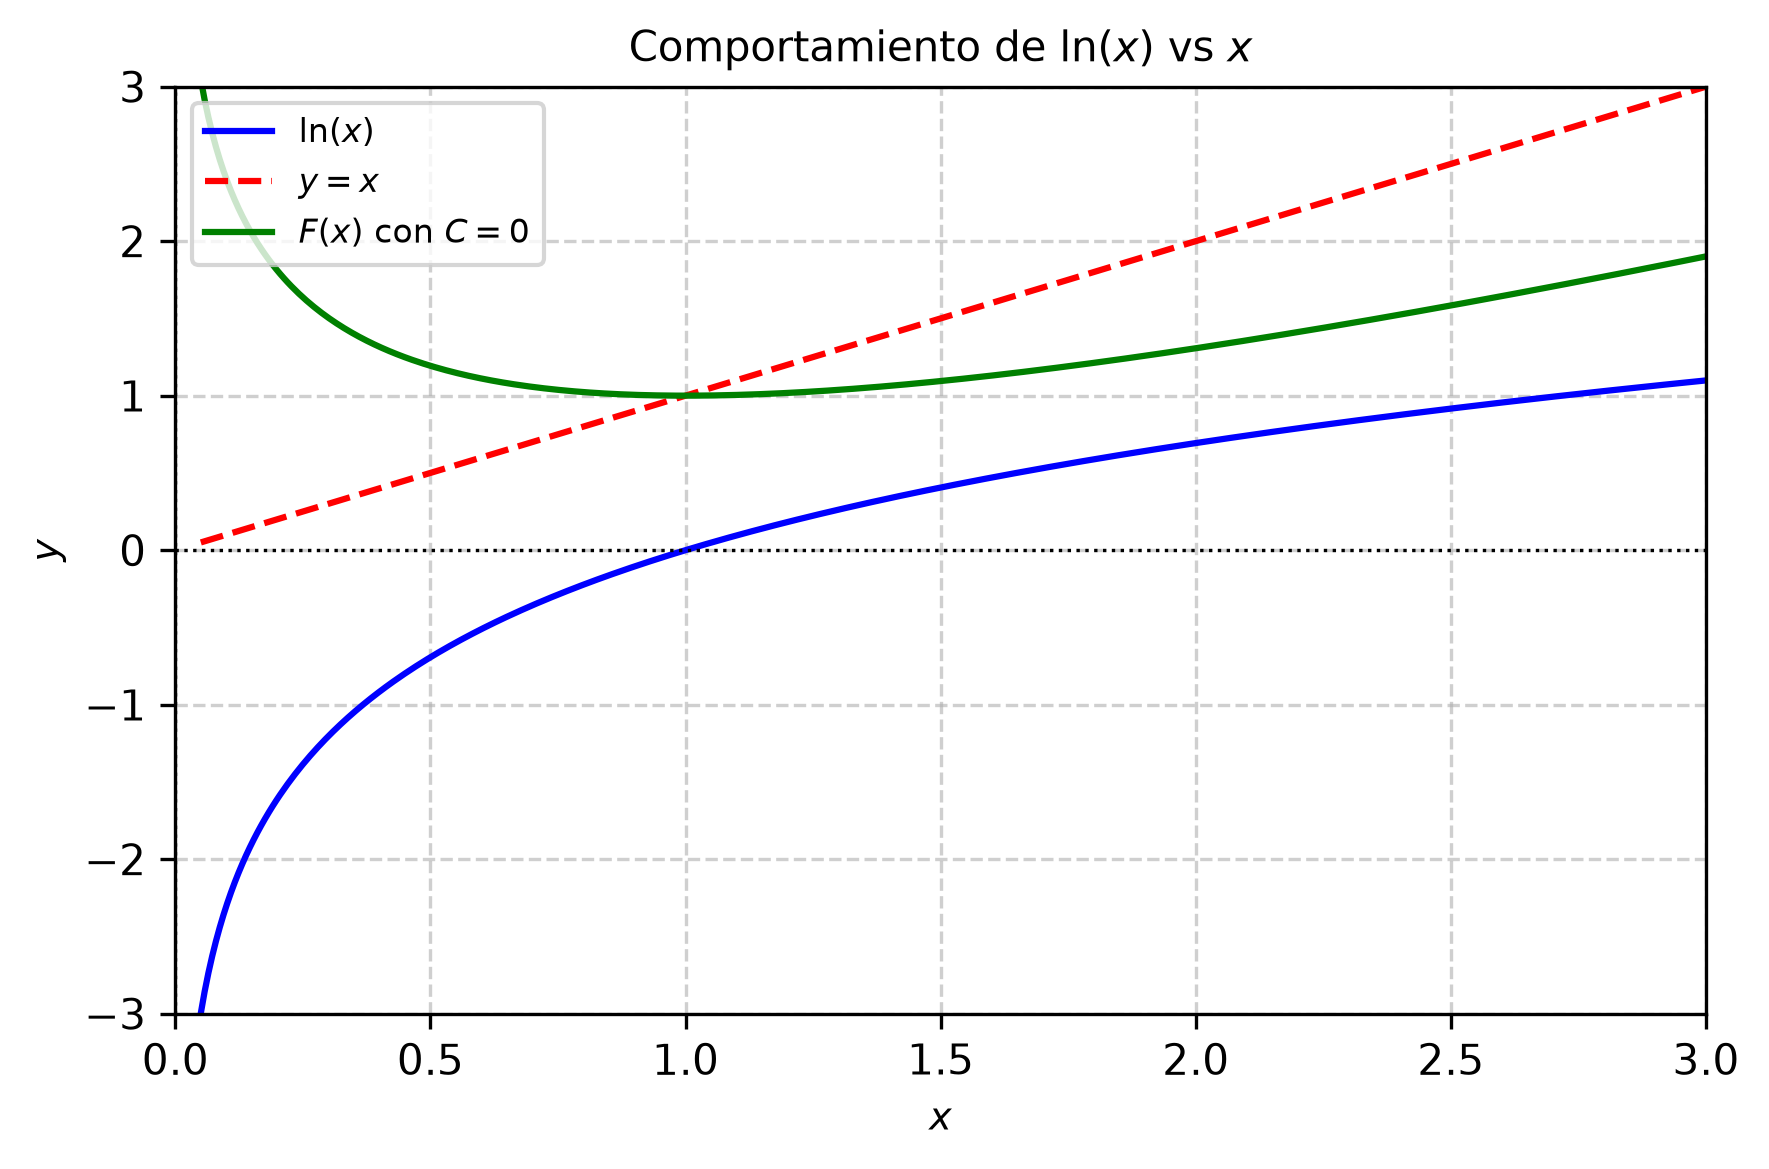
\includegraphics[width=\columnwidth]{semana_08/graficas/estesi.png}
    \caption{Representación gráfica de las funciones $\ln(x)$, $y=x$ y $f(x) = x - \ln(x)$ (Problema 02).}
    \label{fig:problema02}
\end{figure}

	\subsection*{Problema 03}

\textbf{Enunciado:} Probar que si $0 < x < y$, 
entonces se cumple la desigualdad:
\begin{equation*}
\dfrac{1}{y} < \dfrac{\ln y - \ln x}{y - x} < \dfrac{1}{x}
\end{equation*}

\textbf{Solución:} 
Para demostrar la desigualdad propuesta, 
utilizamos el Teorema del Valor Medio 
de Lagrange. 

Consideremos la función real 
$f(t) = \ln(t)$. 
Esta función es continua en el intervalo 
cerrado $[x, y]$ y derivable en el 
intervalo abierto $(x, y)$, 
dado que $0 < x < y$.

Por el Teorema del Valor Medio, 
existe al menos un número $c$ en el 
intervalo $(x, y)$ tal que:
\begin{align*}
f'(c) &= \dfrac{f(y) - f(x)}{y - x}
\end{align*}

Calculamos la derivada de la función 
$f(t)$:
\begin{align*}
f'(t) &= \dfrac{1}{t}
\end{align*}

Evaluando la derivada en el punto $c$, 
obtenemos $f'(c) = \dfrac{1}{c}$. 
Sustituyendo esto en la expresión del 
teorema, junto con $f(y) = \ln(y)$ y 
$f(x) = \ln(x)$, resulta:
\begin{align*}
\dfrac{1}{c} &= \dfrac{\ln y - \ln x}{y - x}
\end{align*}

Como se sabe que el valor $c$ pertenece 
al intervalo abierto $(x, y)$, 
se cumple la siguiente desigualdad 
estricta para sus inversos:
\begin{align*}
x < c < y \implies \dfrac{1}{y} < \dfrac{1}{c} < \dfrac{1}{x}
\end{align*}

Finalmente, sustituyendo la expresión 
de la derivada evaluada en $c$ dentro 
de esta cadena de desigualdades, 
obtenemos el resultado deseado:
\begin{align*}
\dfrac{1}{y} < \dfrac{\ln y - \ln x}{y - x} < \dfrac{1}{x}
\end{align*}
Esto completa la demostración.

\begin{figure}[H]
	\centering
	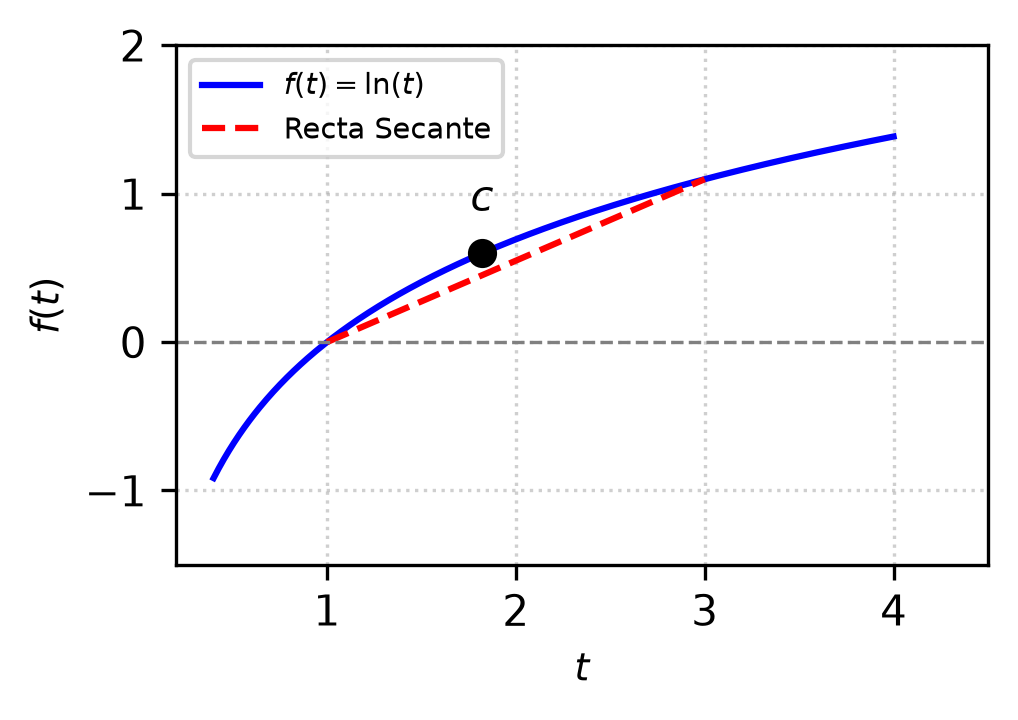
\includegraphics[width=\columnwidth]{semana_08/graficas/SEM08_P03_grafica.png}
	\caption{Representación gráfica de $f(x)$ y su antiderivada $F(x)$ evaluada para la constante de integración $C = 0$ (Problema 03).}
	\label{fig:problema03}
\end{figure}

	\subsection*{Problema 04}

\textbf{Enunciado:}
Probar que para todo entero $n \ge 2$:
\begin{align*}
\sum_{k=2}^{n} \dfrac{1}{k} < \ln(n) < \sum_{k=1}^{n-1} \dfrac{1}{k}
\end{align*}

\textbf{Solución:}
La función $f(t) = \dfrac{1}{t}$ es continua y decreciente en el intervalo $[1, \infty)$. 
Sabemos que el logaritmo natural se define mediante la integral:
\begin{align*}
\ln(n) = \int_{1}^{n} \dfrac{1}{t} \, dt
\end{align*}

Podemos aproximar esta integral mediante sumas de Riemann usando una partición regular del intervalo $[1, n]$ con subintervalos de ancho $\Delta t = 1$, cuyos puntos extremos son $t_k = k$ para $k = 0, 1, 2, \dots, n$.

Para la cota inferior, consideramos los rectángulos inscritos (suma inferior) en cada subintervalo $[k, k+1]$ con altura dada por el extremo derecho $f(k+1) = \dfrac{1}{k+1}$:
\begin{align*}
\int_{1}^{n} \dfrac{1}{t} \, dt &> \sum_{k=1}^{n-1} f(k+1) \cdot \Delta t \\
\int_{1}^{n} \dfrac{1}{t} \, dt &> \sum_{k=1}^{n-1} \dfrac{1}{k+1}
\end{align*}

Cambiando el índice con $j = k+1$, la suma de la derecha se reescribe como:
\begin{align*}
\sum_{j=2}^{n} \dfrac{1}{j} = \dfrac{1}{2} + \dfrac{1}{3} + \dots + \dfrac{1}{n}
\end{align*}
Esto demuestra la primera parte de la desigualdad.

Para la cota superior, consideramos los rectángulos circunscritos (suma superior) en cada subintervalo $[k, k+1]$ con altura dada por el extremo izquierdo $f(k) = \dfrac{1}{k}$:
\begin{align*}
\int_{1}^{n} \dfrac{1}{t} \, dt &< \sum_{k=1}^{n-1} f(k) \cdot \Delta t \\
\int_{1}^{n} \dfrac{1}{t} \, dt &< \sum_{k=1}^{n-1} \dfrac{1}{k}
\end{align*}

Desarrollando esta última suma, obtenemos:
\begin{align*}
\ln(n) < 1 + \dfrac{1}{2} + \dots + \dfrac{1}{n-1}
\end{align*}

Combinando ambos resultados, queda demostrado que:
\begin{align*}
\sum_{k=2}^{n} \dfrac{1}{k} < \ln(n) < \sum_{k=1}^{n-1} \dfrac{1}{k}
\end{align*}
Quedando establecida la relación geométrica entre las sumas armónicas y la función logarítmica.

\begin{figure}[H]
	\centering
	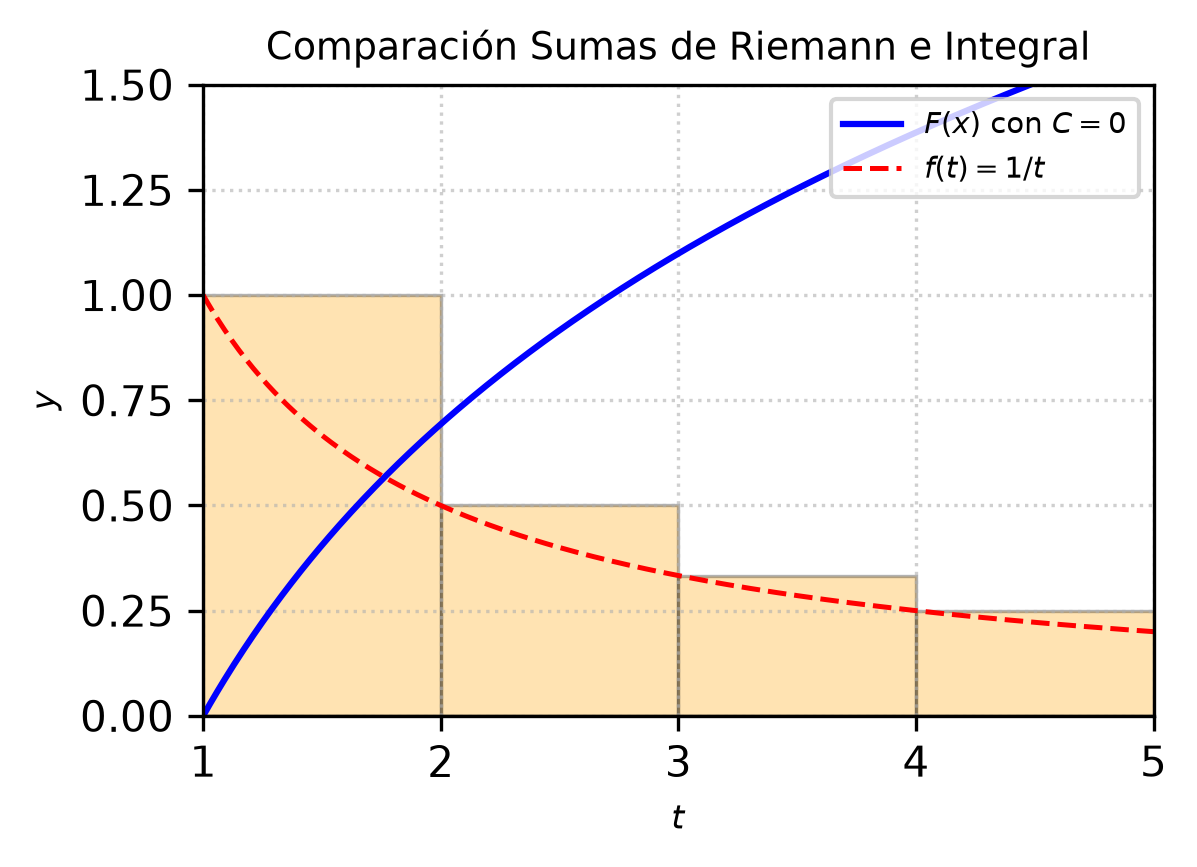
\includegraphics[width=\columnwidth]{semana_08/graficas/SEM08_P04_grafica.png}
	\caption{Representación gráfica de $f(x)$ y su antiderivada $F(x)$ evaluada para la constante de integración $C = 0$ (Problema 04).}
	\label{fig:problema04}
\end{figure}

\end{document}